\documentclass[a4paper,12pt]{article}
\usepackage{amsmath,amssymb,amsfonts,amsthm}
\usepackage{tikz}
\usepackage[utf8x]{inputenc}
\usepackage[T2A]{fontenc} 
\usepackage[russian]{babel}
\usepackage{cmap} 
\usepackage{ gensymb }
% Так ссылки в PDF будут активны
\usepackage[unicode]{hyperref}
\usepackage{ textcomp }
\usepackage{indentfirst}
\usepackage[version=3]{mhchem}

% вы сможете вставлять картинки командой \includegraphics[width=0.7\textwidth]{ИМЯ ФАЙЛА}
% получается подключать, как минимум, файлы .pdf, .jpg, .png.
\usepackage{graphicx}
% Если вы хотите явно указать поля:
\usepackage[margin=1in]{geometry}
% Или если вы хотите задать поля менее явно (чем больше DIV, тем больше места под текст):
% \usepackage[DIV=10]{typearea}

\usepackage{fancyhdr}

\newcommand{\bbR}{\mathbb R}%теперь вместо длинной команды \mathbb R (множество вещественных чисел) можно писать короткую запись \bbR. Вместо \bbR вы можете вписать любую строчку букв, которая начинается с '\'.
\newcommand{\eps}{\varepsilon}
\newcommand{\bbN}{\mathbb N}
\newcommand{\dif}{\mathrm{d}}

\newtheorem{Def}{Определение}


\pagestyle{fancy}
\makeatletter % сделать "@" "буквой", а не "спецсимволом" - можно использовать "служебные" команды, содержащие @ в названии
\fancyhead[L]{\footnotesize }%Это будет написано вверху страницы слева
\fancyhead[R]{\footnotesize ФУПМ МФТИ}
\fancyfoot[L]{\footnotesize \@author}%имя автора будет написано внизу страницы слева
\fancyfoot[R]{\thepage}%номер страницы —- внизу справа
\fancyfoot[C]{}%по центру внизу страницы пусто

\renewcommand{\maketitle}{%
	\noindent{\bfseries\scshape\large\@title\ \mdseries\upshape}\par
	\noindent {\large\itshape\@author}
	\vskip 2ex}
\makeatother
\def\dd#1#2{\frac{\partial#1}{\partial#2}}


\title{2.2 \\ Изучение спектров атомов водорода и дейтерия}
\author{Северилов Павел, 674} 
\date{03 декабря 2018 г.}

\begin{document}
		\maketitle
		
		
	\paragraph{Цель работы:} Исследовать спектральные закономерности в оптических спектрах водорода и дейтерия. По результатам измерений вычислить постоянные Ридберга для этих двух изотопов водорода, их потенциалы ионизации, изотопические сдвиги линий.
	
	\section{Теория}
	\subsection{Атомарный спектр}
	Длины волн спектральных линий водородоподобного атома описывается формулой:
	\begin{equation} \label{balmer}
	\frac{1}{\lambda_{mn}} = R Z^2 \left( \frac{1}{n^2} - \frac{1}{m^2} \right),
	\end{equation}
	
	где $R$~---~константа, называемая постоянной Ридберга, а $m$ и $n$~---~целые числа.
	
	Формула (\ref{balmer}) известна в спектроскопии очень давно. Она была выведена эмпирически и называна \textit{обобщенной формулой Бальмера}. Эта формула достаточно точно описывает спектральные линии водорода при $R = 109677.6 \; cm^{-1}$. Однако физический смысл формулы был непонятен в то время.
	
	Для объяснения спектра атома водорода Нильс Бор в 1913г. предложил теорию атома, в основу которой положил три постулата:
	\begin{enumerate}
		\item Из всех возможных с точки зрения классической физики орбит в атоме осуществляются только некоторые стационарные орбиты, при движении по которым, вопреки представлениям классической электродинамики, электрон не излучает энергии.
		\item Из всех возможных орбит в атоме осуществляются только те, для которых момент количества движения равен целому кратному величины постоянной Планка $\hbar~=~h/2\pi$, т.е. 
		\begin{equation}
		L = n \hbar
		\end{equation}
		\item Излучение или поглощение энергии происходит при переходе атома из одного стационарного состояния в другое, а частота излучаемого (поглощаемого) света связана с разностью энергий атома в стационарных состояниях соотношением 
		\begin{equation}
		h \nu = E_2 - E_1,
		\end{equation}
		где $\nu$~--~частота излучаемой линии.
	\end{enumerate}
	
	\begin{figure}[ht!]
		\label{series}
		\centering
		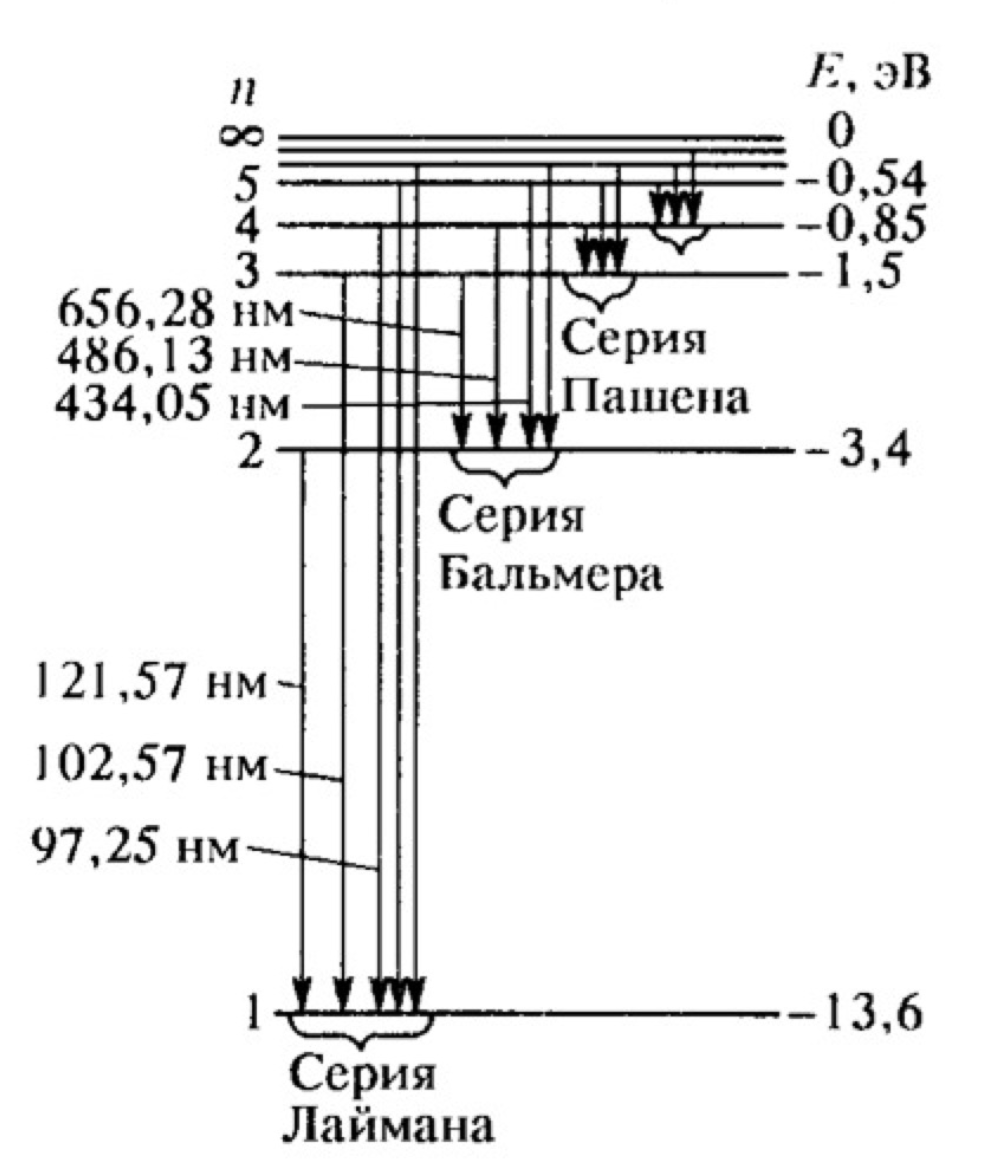
\includegraphics[width=.4\linewidth]{./img/series.png}
		\caption{Уровни энергии атома водорода и образование спектральных серий}
	\end{figure}
	
	Использование этих постулатов с учетом кулоновского взаимодействия между ядром и электроном позволяет легко определить возможные энергетические состояния водородоподобного атома. Если считать ядро неподвижным, то эти энергетические состояния определяются выражением 
	\begin{equation} \label{energy}
	E_n = - \frac{2 \pi^2 m_e e^4 Z^2}{h^2} \frac{1}{n^2} \equiv -RZ^2 \frac{1}{n^2}
	\end{equation}
	
	Знание энергетических состояний атома позволяет в соответствии с формулой (\ref{energy}) определить возможные частоты его излучения и объяснить наблюдаемые спектральные  закономерности (см. рис. \ref{series}). 
	
	\subsection{Молекулярный спектр}
	Молекулы обладают более богатым спектром возбужденных состояний, чем изолированные атомы. В то время как возбуждения атомов -- это переходы их электронов на более высоко расположенные энергетические уровни, в молекулах могут возбуждаться дополнительно колебательные степени свободы: колебания составляющих их атомов друг относительно друга и вращательные, т.е. вращения молекул относительно различных осей. В первом приближении энергия молекулы может быть представлена в виде 
	\begin{equation}
	E = E_\text{эл} + E_\text{колеб} + E_\text{вращ}.
	\end{equation}
	
	Можно получить следующую оценку характерных частот этих колебаний:
	\begin{equation}
	\omega_\text{эл} : \omega_\text{колеб} : \omega_\text{вращ} \approx 1 : 10^{-3} : 10^{-6}
	\end{equation}
	
	Характерная энергия вращательных движений в $10^6$ раз меньше энергии электронных переходов, и поэтому наблюдение вращательных переходов оптическими спектрометрами невозможно. Реально в видимой области наблюдаются электронно-колебательные спектры молекул. В спектре излучения происходит наложение колебательного спектра на электронный, и проявляется это в том, что каждой линии электронного перехода соответствует ряд колебательных линий, образующий полосу. На рис. \ref{levels} схематически изображены энергетические уровни молекулы без учета вращательной структуры.
	
	
	\begin{figure}[ht!]\label{levels} 
		\center{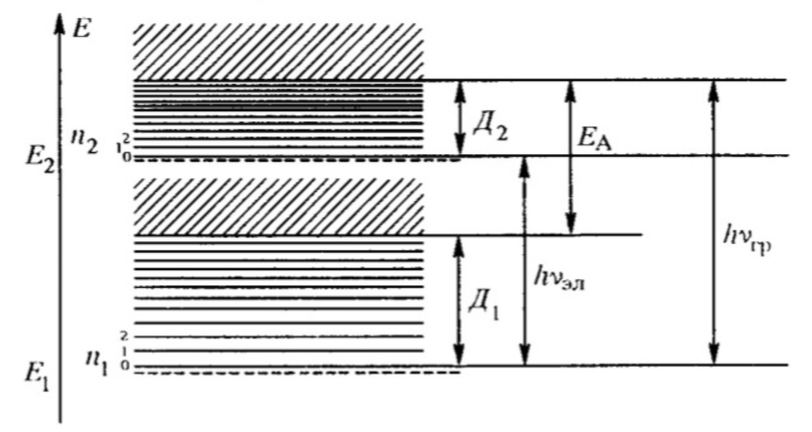
\includegraphics[width=.5\linewidth]{./img/levels.png}}
		\caption{Электронные и электронно-колебательные энергетические уровни двухатомной молекулы}
	\end{figure}
	
	
	\section{Установка}
	Для исследования атомарного спектра водорода и молекулярного спектра йода в работе используется призменный монохроматор УМ-2.
	
	\begin{figure}[ht!]\label{monochrome} 
		\center{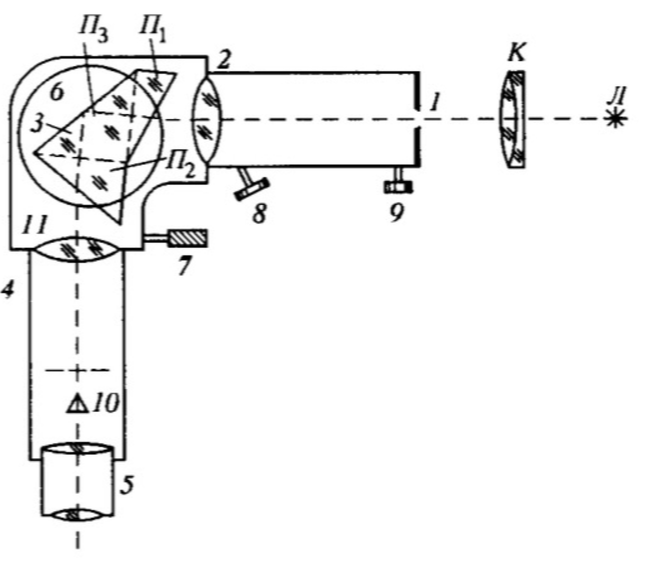
\includegraphics[width=.5\linewidth]{./img/monochrome.png}}
		\caption{Схема УМ-2}
	\end{figure}
	
	Основные части монохроматора:
	\begin{enumerate}
		\item Входная щель 1, снабженная микрометрическим винтом 9.
		\item Коллиматорный объектив 2, снабженный микрометрическим винтом 8.
		\item Сложная призма 3, установленная на поворотном столике 6.
		\item Поворотный столик 6, вращающийся вокруг вертикальный при помощи микрометрического винта 7 с отсчетным барабаном.
		\item Зрительная руба, состоящая из объектива 4 и окуляра 5.
	\end{enumerate}
	
	Монохроматор калибруется с помощью неоновой и ртутной ламп.
	
	\subsection{Спектр атома водорода}
	
	В качестве источника света используется водородная лампа. С помощью монохроматора измеряются линии оптического диапазона из спектра \textit{излучения} водорода (из серии Бальмера).
	
	\newpage
	
	\subsection{Молекулярный спектр йода}
	
	\begin{figure}[ht!]\label{ischeme} 
		\center{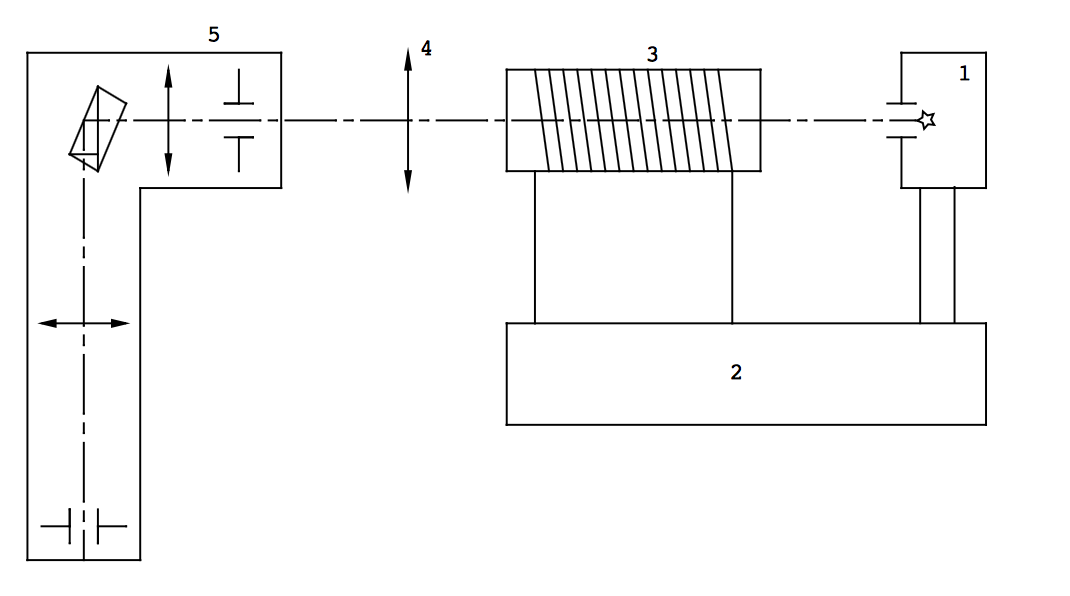
\includegraphics[width=.5\linewidth]{./img/ischeme.png}}
		\caption{Схема установки для исследования спектра йода}
	\end{figure}
	
	Спектр \textit{поглощения} паров йода наблюдается визуально на фоне непрерывного спектра лампы 1.
	
	\section{Обработка результатов}
	
	\begin{enumerate}
		\item Градуировка монохроматора:
		
		\begin{figure}[ht!]\label{grade} 
			\center{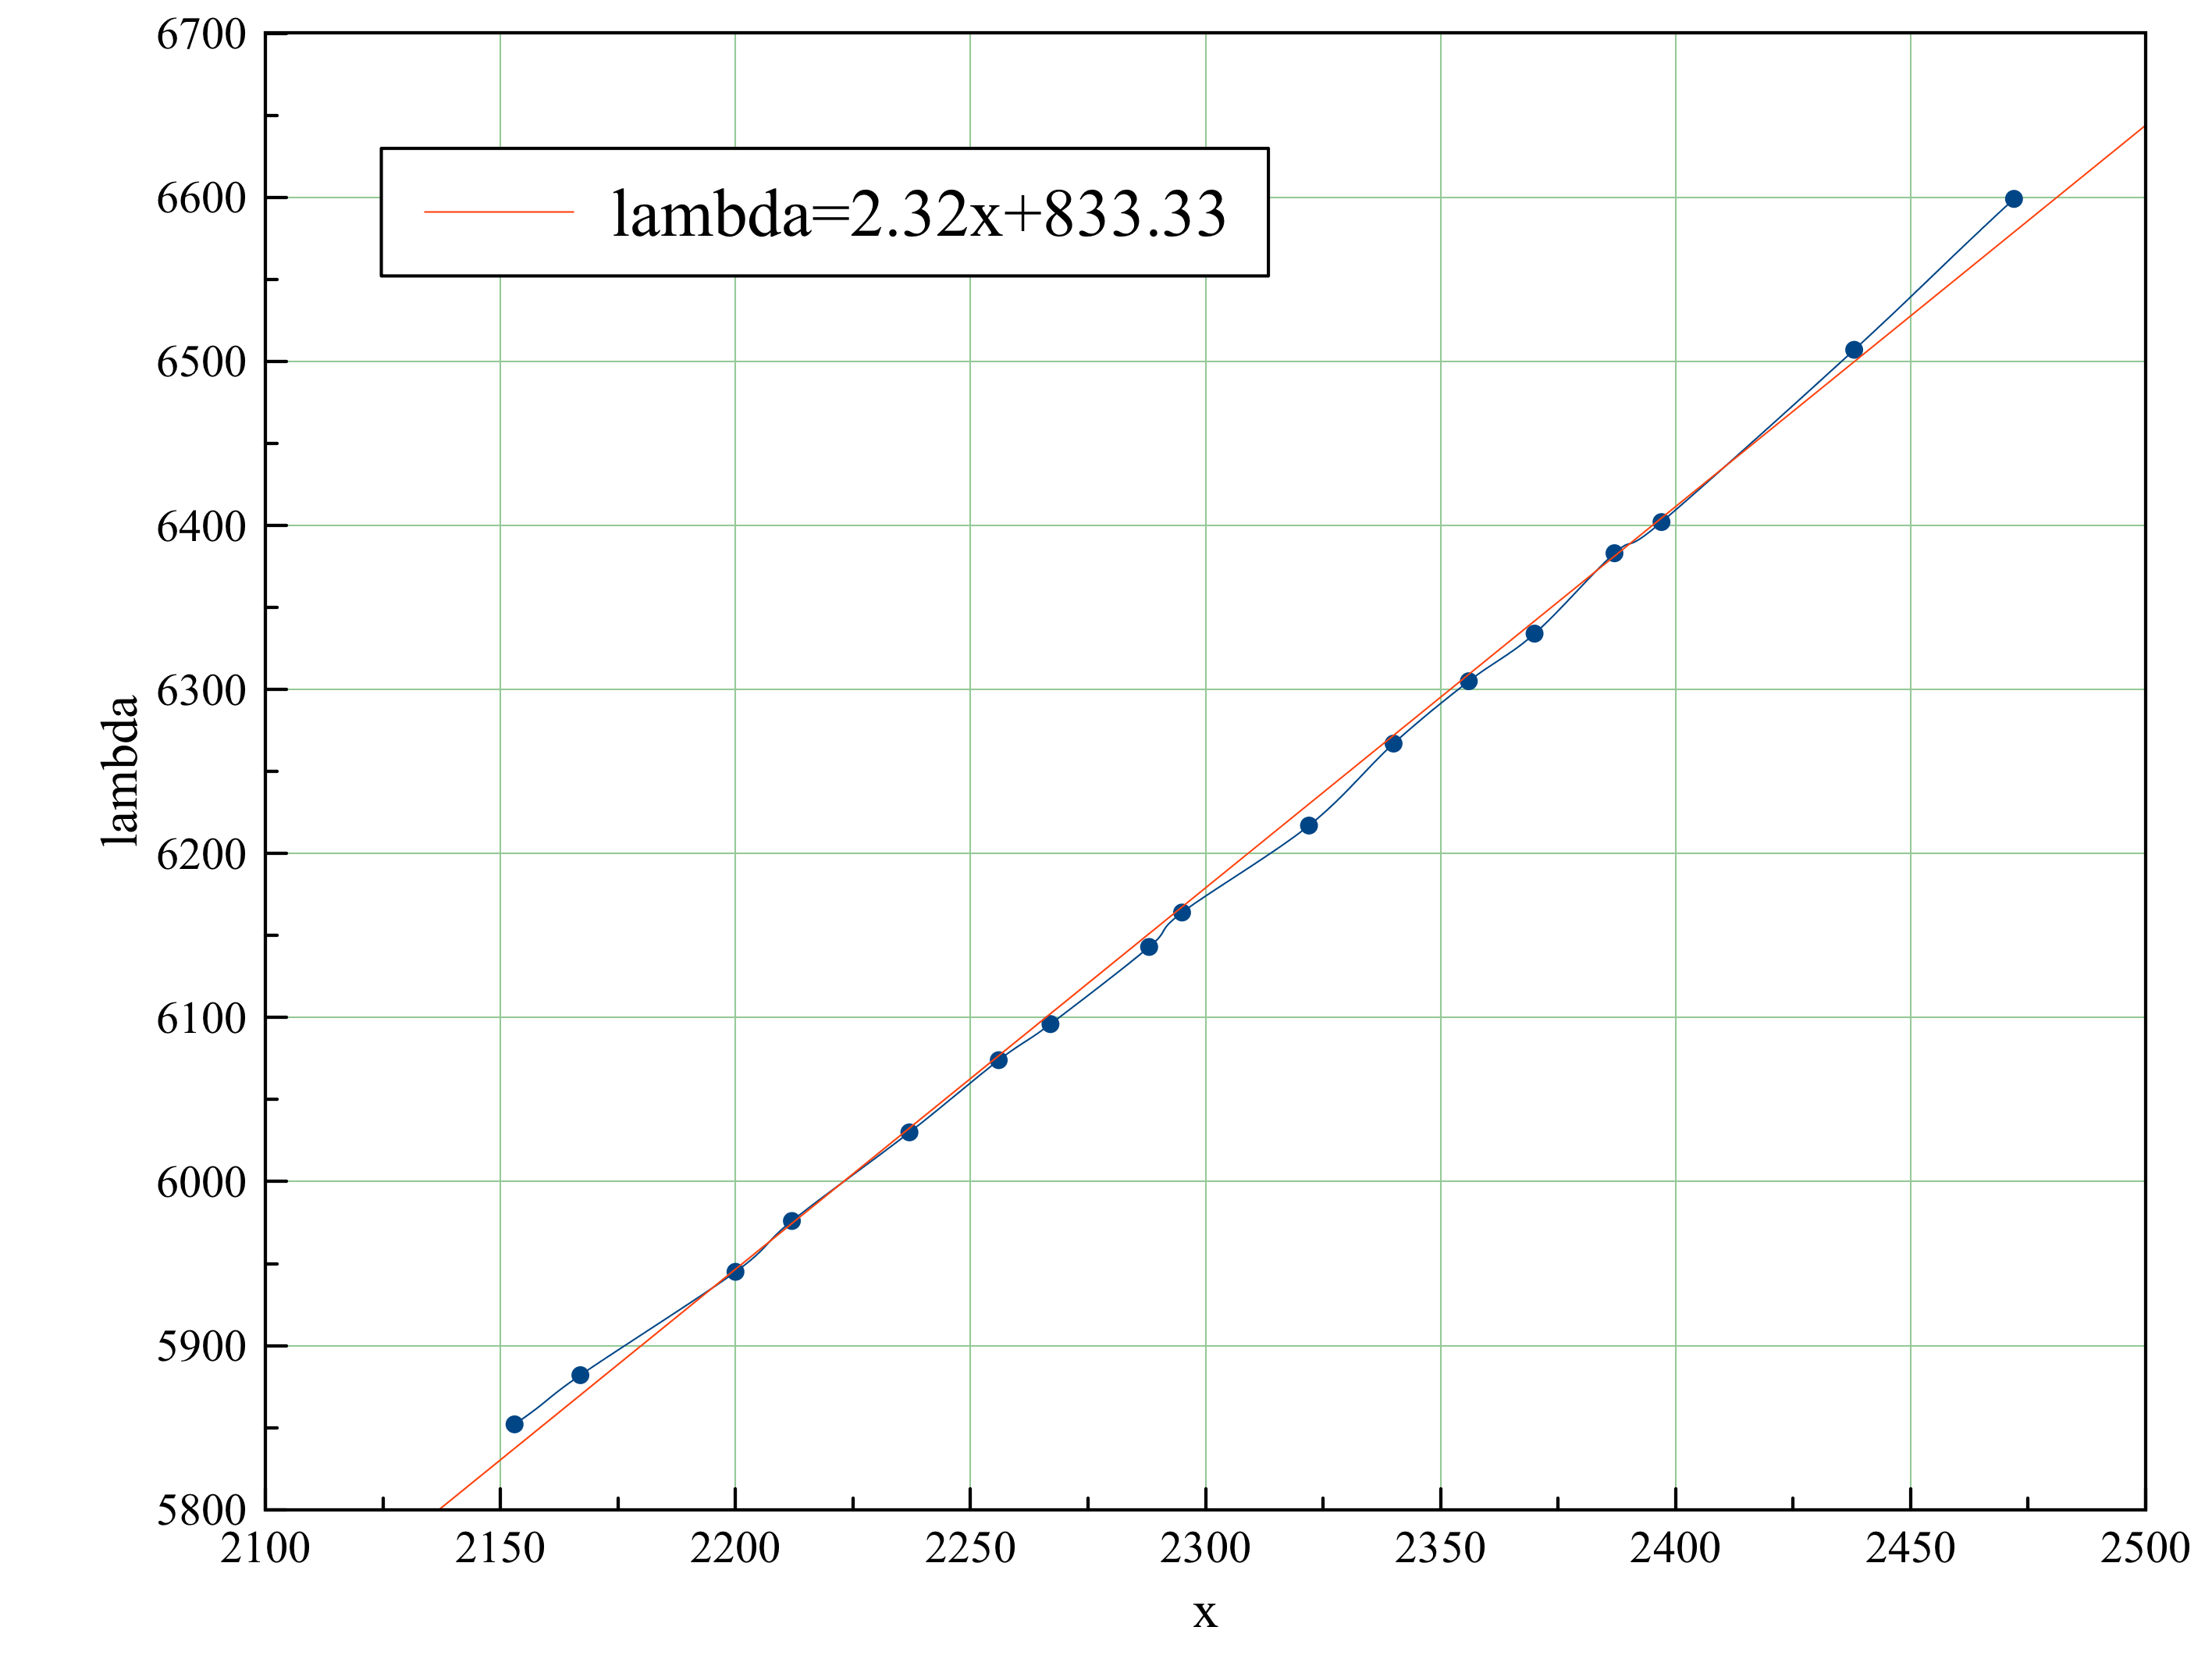
\includegraphics[height=50ex]{./img/grad.png}}
			\caption{Градуировочная кривая}
		\end{figure}
		
		\item Определим координаты линий бальмеровской серии атомарного водорода:
		
		
		\begin{center}
			\begin{tabular}{|c|c|c|c|c|}
				\hline
				Линия & Монохроматор & Длина волны, нм & Справочное значениe, нм & $R, \; 10^{-6}m^{-1}$\\ \hline
				$H_\alpha$ & $2456^o$ & $ 650.3 $ & $ 656.3 $ & $11.0718$ \\ \hline
				$H_\beta$ & $1452^o$ & $ 490.8 $ & $ 486.1$ & $10.8667$ \\ \hline
				$H_\gamma$ & $892^o$ & $407.4 $ & $ 434.1$ & $11.688$ \\ \hline
			\end{tabular}
		\end{center}
		\[\sigma_\lambda = 1.5 \; nm \]
		
		Убедимся, что отношение длин волн водородных линий соответствует формуле сериальной закономерности:
		\[
		\dfrac{H_\alpha}{H_\beta} = 1.325 \approx 1.350 = \dfrac{\frac{1}{2^2}-\frac{1}{4^2}}{\frac{1}{2^2}-\frac{1}{3^2}}
		\qquad
		\dfrac{H_\beta}{H_\gamma} = 1.2 \approx 1.120 = \dfrac{\frac{1}{2^2}-\frac{1}{5^2}}{\frac{1}{2^2}-\frac{1}{4^2}}
		\]
		
		Вычислим постоянную Ридберга:
		\[R = (11.2  \pm 0.1)\cdot 10^{-6} \; m^{-1}\]
		
		\item Вычисление энергии колебательного кванта молекулы йода и энергии ее диссоциации:
		
		\begin{center}
			\begin{tabular}{|c|c|c|}
				\hline
				Линия & Монохроматор & Длина волны, нм \\ \hline
				$h \nu_{1,0}$ 	   	& $2255^o$ & $ 606.5 $ \\ \hline
				$h \nu_{1,5}$ 	   	& $2173^o$ & $ 587.5 $  \\ \hline
				$h \nu_\text{гр}$ 	& $2354^o$ & $ 629.5 $ \\ \hline
			\end{tabular}
		\end{center}
		\[\sigma_\lambda = 1.5 \; nm\]
		
		\begin{itemize}
			
			\item Энергия колебательного кванта:
			\[h \nu_2 = \dfrac{h \nu_{1,5} - h \nu_{1,0}}{5} = 13.2 \pm 0.5 \; m eV \]
			
			\item Энергия электронного перехода:
			\[h \nu_\text{эл} = h \nu_{1} - \nu_2 = (1.38 \pm 0.10)1-^{-2} \; eV \]
			
			\item Энергия диссоциации молекулы в основном состоянии $\text{Д}_1$:
			\[ D_1 = h \nu_\text{гр} - E_A = 1.13 \pm 0.10 \; eV \]
			
			\item Энергия диссоциации молекулы в возбужденном состоянии $\text{Д}_2$:
			\[ D_2 = h \nu_\text{гр} - h \nu_\text{эл} = 2.053 \pm 0.108 \; eV \]
			
		\end{itemize}
		
	\end{enumerate}
	
	\section{Вывод}
	В ходе эксперимента были исследованы спектры водорода и йода. Из формулы (\ref{balmer}) была вычислена постоянная Ридберга:
	\[
	R_\text{эксп} = (11.2  \pm 0.1)\cdot 10^{-6} \; m^{-1}
	\qquad
	R_\text{теор} = 10.9737\cdot 10^{-6} \; m^{-1}
	\]
	Были исследованы энергии различных состояний молекулы йода:
	\begin{itemize}
		
		\item Энергия колебательного кванта:
		\[h \nu_2 = 13.2 \pm 0.5 \; m eV \]
	\[(h \nu_1 = 27 \; m eV ; ~~E_A = 0.94 \; eV) \]
		
		\item Энергия электронного перехода:
		\[ h \nu_\text{эл} = (1.38 \pm 0.10)\cdot 10^{-2} \; eV \]
		
		\item Энергия диссоциации:
		\[
		D_1 = 1.13 \pm 0.10 \; eV
		\qquad
		D_2 = 2.053 \pm 0.108 \; eV 
		\]
	\end{itemize}
	
	Все полученные значения выглядят достоверно: постоянная Ридберга совпадает с табличным значением с точностью до погрешности, энергии колебательного кванта совпадают по порядку величины, энергия диссоциации близка к термохимическим данным.

\end{document}
